\chapter{Prescriptive analysis}{}

%citazione introduttiva
\epigraph{\textit{Aren’t we doctor, after all?}}{}

All the previous chapters of this mathematical section, introduced methods to describe and understand a dataset, and even to create knowledge by discovering hidden patterns within data.\par

When the decision-maker has a clear description of the processes, it is necessary to find decision-support methods to leave a footprint in the real world. This should be the last stage of any serious data-driven process since starting building a decision support tool without a clear idea of the process where it is going to be embedded may lead to catastrophic results.\par

Besides, it is important to remember that statistics and learning algorithms provide much information. Sometimes, this information is enough for making a decision without additional biases introduced by complex decision-support tools.\par

It is important to remember that prescriptive models are highly complex and incredibly problem-oriented. This fact suggests that they usually embed the highest bias possible and a limited generalisation of their mechanism, which also prevents their repeatability and their value for academics.\par

\section{Prescriptive models}
Prescriptive models aim at setting the value of decision variables that mimic the decision alternatives in a real context. These models are defined using the following notation.

\begin{itemize}
    \item $P$ is the decision problem;
    \item $x$ is the matrix of the decision variables;
    \item $z$ is the objective function explaining the goodness of $x$;
    \item $\xi$ is the domain of $x$.
\end{itemize}

Prescriptive models are algorithms minimising (or maximising) $z$ by changing the entries of $x$ within the domain $\xi$. Prescriptive models outcome are the solution $\hat{x}$ and the solution value $\hat{z}$. Let assume $P$ being a minimisation problem, we define $\hat{x}$:

\begin{itemize}
    \item Optimal solution (indicated with $x^\ast$) if the value of $\hat{z}$ is the minimum among all the possible values of $\hat{z}$;
    \item Feasible solution if $x\in\xi$;
    \item Unfeasible solution if $x\notin\xi$.
\end{itemize}

\section{Heuristics and metaheuristics}
Considering a minimisation problem $P$, a heuristic procedure is any algorithm that produces a feasible solution $\hat{x}$ performing different step; each step aims at reducing the value of $z$. Each step of a heuristic algorithm is called \textit{move}. Usually, a move of a heuristics produces an improvement (i.e., it reduces the value of $z$), when no improvement occurs the algorithm stops returning the value of $\hat{x}$ and $\hat{z}$. Differently, a metaheuristic algorithm allows accepting bad values of $z$ at the intermediate moves of the algorithm aiming at a lower value of $z$ in the last move. Figure \ref{fig_heurMetaheur} presents the typical behaviour of the moves of heuristics and metaheuristics algorithms.


% INSERT fig_heurMetaheur
\begin{figure}[hbt!]
\centering
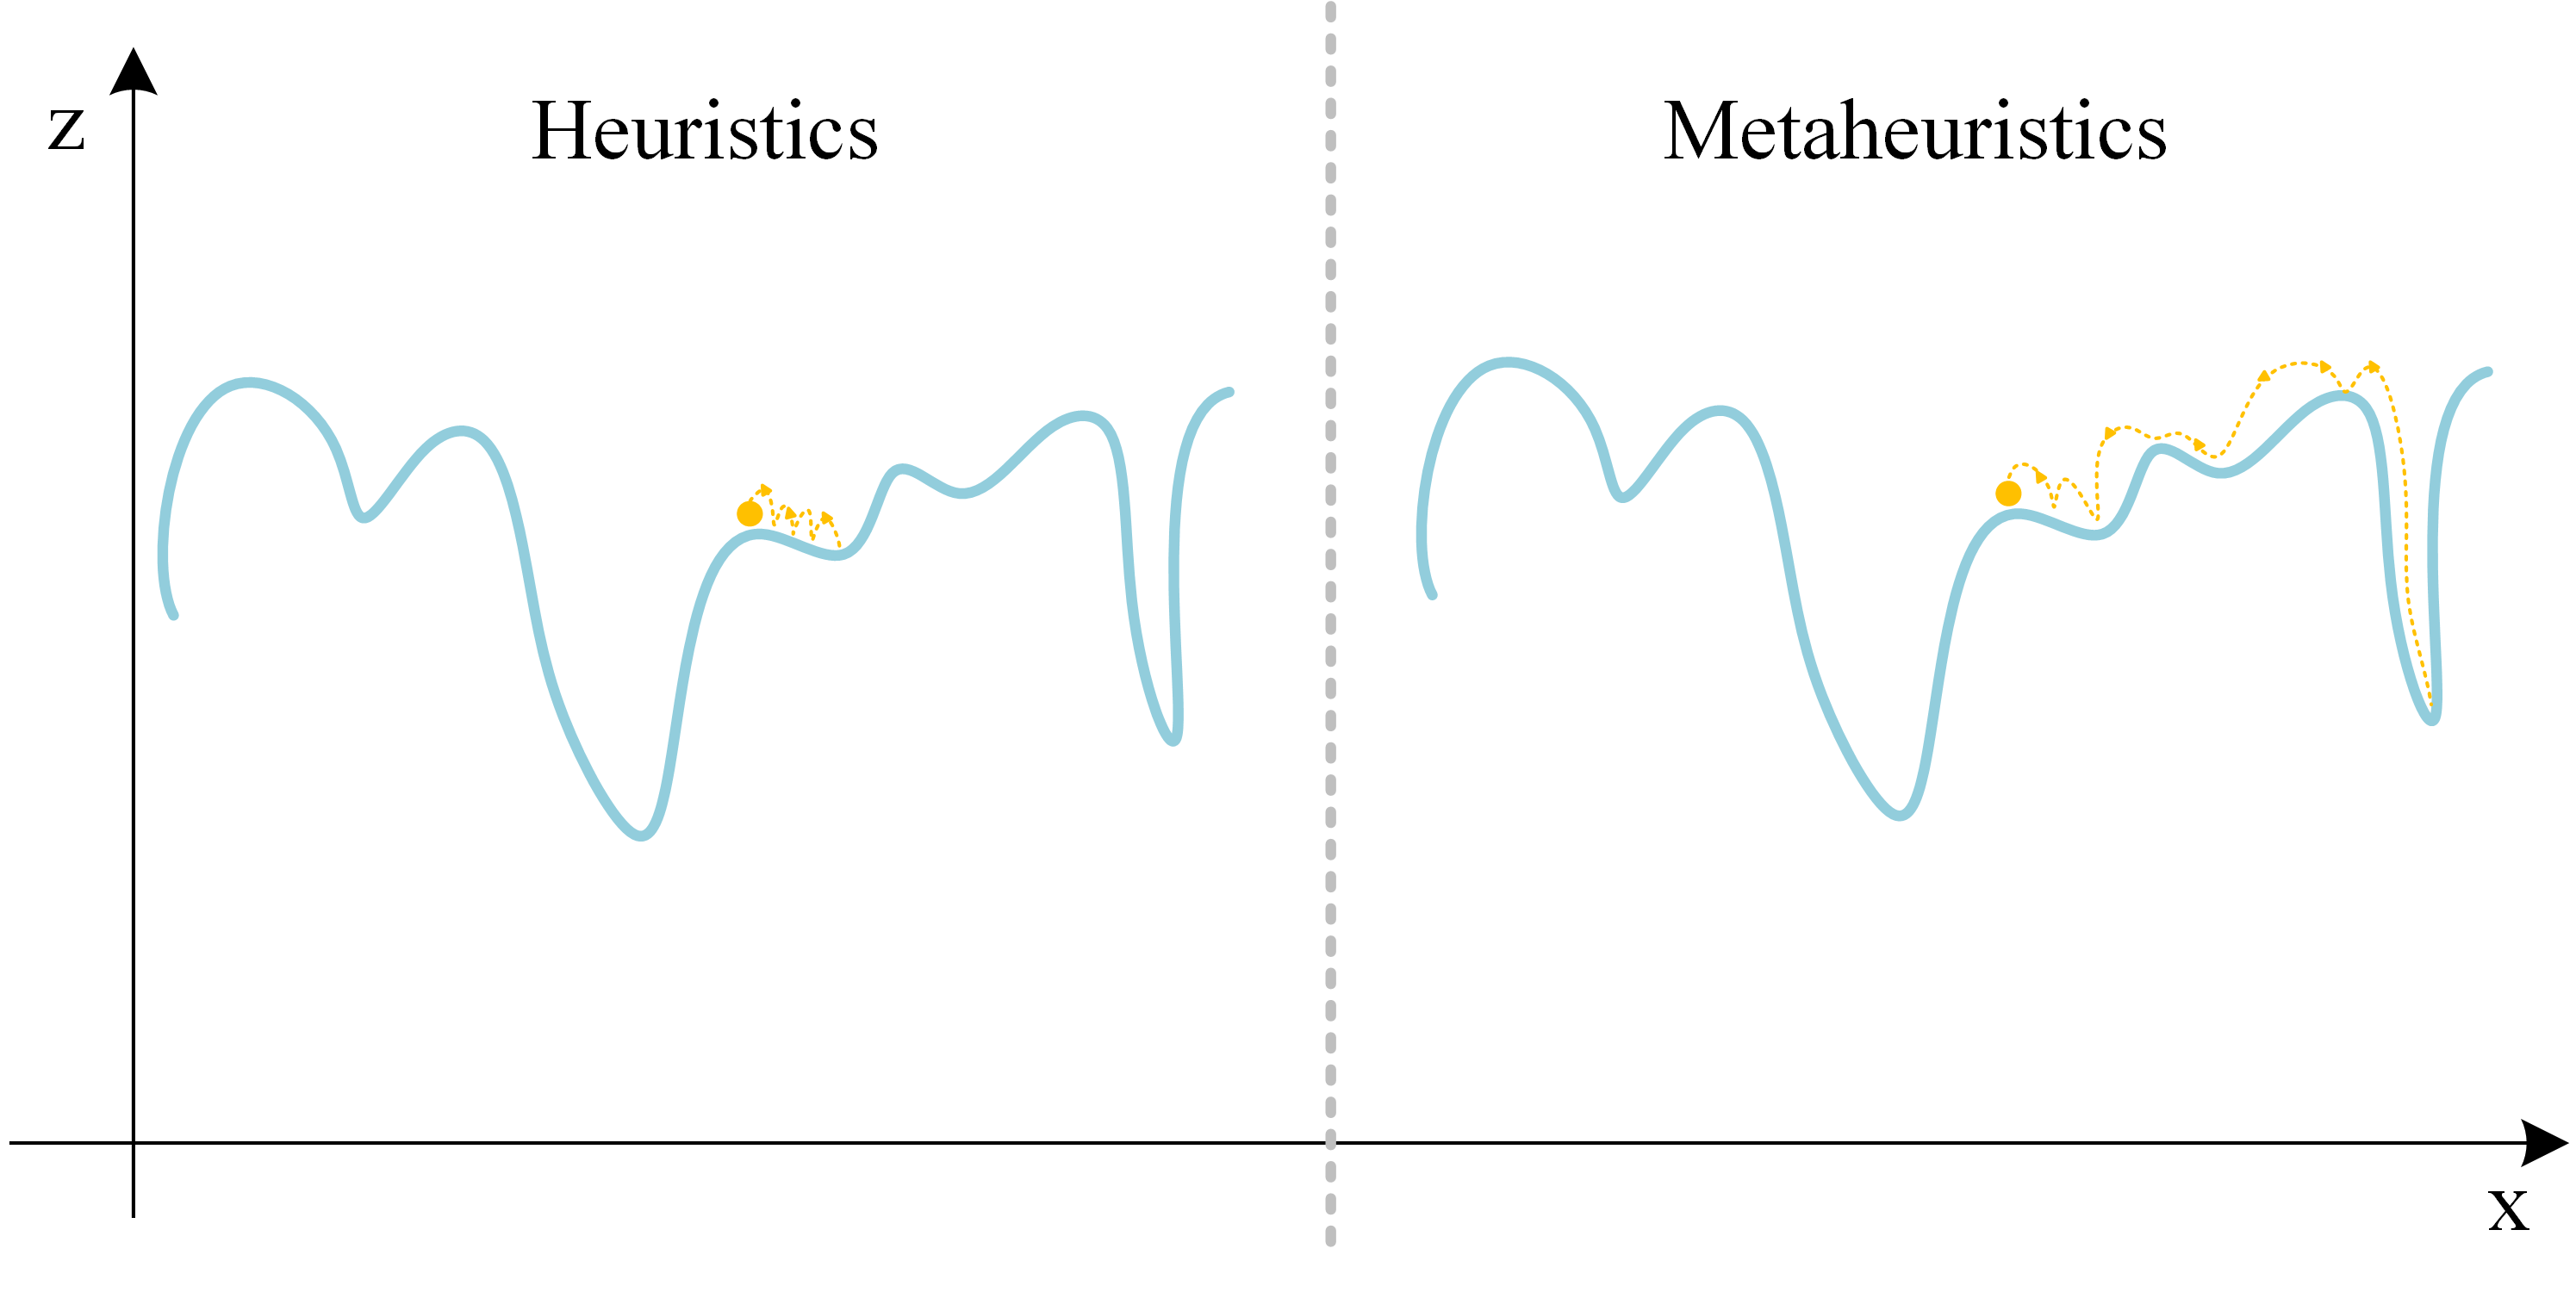
\includegraphics[width=0.9\textwidth]{SectionLetsMath/prescriptive_fig/fig_heurMetaheur.png}
\captionsetup{type=figure}
\caption{Representation of the moves of heuristics and metaheuristics algorithms.}
\label{fig_heurMetaheur}
\end{figure}

Heuristics can be:

\begin{itemize}
    \item Greedy algorithms, i.e. they perform a number of steps to build a feasible solution;
    \item Local search, i.e. they perform a number of steps to improve an initial feasible solution.
\end{itemize}

Metaheuristics usually start from a feasible solution (e.g. produced by a greedy algorithm), and they perform a number of moves according to the type of the algorithm. Examples of metaheuristics algorithms are simulated annealing, tabu search, ant colony algorithm, genetic algorithm (see section \ref{geneticSearch}). Each of them has a precise logic to generate the solution at each step, it checks (or recovers) the feasibility of the incumbent solution within $\xi$ improving $z$.

\section{Linear Optimisation}

Heuristics and metaheuristics hardly guarantee to find the optimal $x^\ast$ and $z^\ast$. Linear optimisation uses predefined algorithms to find the optimal solution to a linear problem $P$ having $\xi$ defined by linear constraints. An optimisation problem can be written in the form:

\begin{equation}
\begin{split}
    z=\min{c^\prime x} \\
    Ax\le b \\
    x\geq0 \\
\end{split}
\label{eq_linearProblem}
\end{equation}

If $\xi$ is a continuous domain, $P$ is a linear problem (LP) and can be solved in polynomial time using the simplex algorithm. If $\xi$ is made of integer values, the problem is an integer linear problem (ILP), and it is solvable in exponential time using the branch \& bound algorithm. Exponential time may take forever to solve an instance; for this reason, ILP optimisation is not suitable for big instance of problems requiring real-time response. In the next paragraph, we introduce some algorithms (still having an exponential complexity) which can improve the running time to get an optimal solution.

\subsection{Duality} \label{secDuality}

We can find a smart way to compute the optimal solution of an optimisation problem $P$, by considering its dual problem $D$.\par

Let consider a primal problem $P$ defined as:
\begin{equation}
\begin{split}
    z=\min{c^\prime x}\\
    Ax\le b\\
    x\geq0\\
\end{split}
\label{eq_primalProblem1}
\end{equation}
The optimal solution value $z$ of the problem $P$ is obtained at $c^\prime x^\ast$.\par 

Let consider the Lagrangian relaxation $L$ of the problem $P$, where the set of constraints $Ax\le b$ is replaced by a penalty addendum $p\prime\left(b-Ax\right)$ in the objective function.
\begin{equation}
\begin{split}
    \min{c^\prime x-p\prime(b-Ax)}\\
    x\geq0\\
\end{split}
\label{eq_lagrangianRelaxation}
\end{equation}

Let $g(p)$ be the solution value of the relaxed problem $L$. $g(p)$ is a lower bound of $c\prime x$.

\begin{equation}
g\left(p\right)\le c\prime x
\label{eq_lagrangianRelaxationSolutionValue}
\end{equation}

Equation (\ref{eq_lagrangianRelaxationSolutionValue}) implies that it is possible to find a vector $p\prime$ such that $p^\prime\left(b-Ax\right)=0$ obtaining a solution value of the relaxed problem equal to the optimal solution value of the non-relaxed problem. The problem to find $p\prime$ is called dual problem $D$, and it is formally defined as:

\begin{equation}
\begin{split}
    v=\max{p^\prime b}\\
    p\prime A\le c\\
    p\geq0\\
\end{split}
\label{eq_dualProblem}
\end{equation}

A set of mathematical rules from the theorem of duality allows obtaining the definition of the dual problem of any primal problem. Table \ref{tab_duality} illustrates these rules.

% INSERT tab_duality
\begin{figure}[hbt!]
\centering
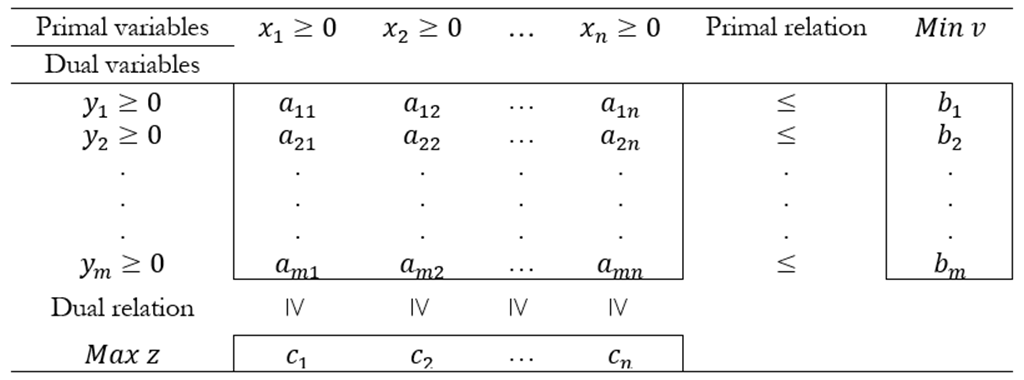
\includegraphics[width=0.9\textwidth]{SectionLetsMath/prescriptive_fig/tab_duality.png}
\captionsetup{type=table}
\caption{Table of the rules to obtain the dual problem.}
\label{tab_duality}
\end{figure}

Sometimes, solving the dual problem is easier than solving the primal problem. In particular, the dual problem can be used to:
\begin{enumerate}
    \item find a lower bound of the solution value of a problem. $g\left(p\right)\le c\prime x$ (e.g. to start a branch \& bound procedure);
    \item generate variables (i.e. columns) for a problem with an exponential number of variables $p\prime\left(b-Ax\right)$ (Branch \& Price algorithm).
\end{enumerate}

\subsubsection{Branch \& price algorithm}
Branch \& price uses the duality theorem to expedite the search of an optimal solution for an ILP problem $P$ having an exponential number of variables. It is a common technique when we express a problem in a set-covering approach, since set covering formulation has an exponential number of variables.\par
Let consider, for example, a facility location problem in its set covering formulation where $w_i$ is the demand of node $i$, and $W$ is the service capacity of a facility. We define the set $S$ as a set of vectors $s$, each one containing a feasible solution of the facility location problem.
\begin{equation}
S=\left\{s\subseteq\left\{i=1,\ldots m\right\}:\sum_{i\in s}{w_i\le W}\right\}
\label{eq_dualProblemSetS}
\end{equation}
We formulate the facility location problem in the form of a set covering problem using  the variable $x_s$, and the parameter $c_s$:

\begin{equation}
	x_s=\left\{
                \begin{array}{ll}
                  1  & if\ configuration\ s\ is\ selected\\
                  0 & otherwise\\
                \end{array}
              \right.\\
\label{eq_dualProblemProblemVariables1}
\end{equation}

\begin{equation}
	c_s\ cost\ of\ serving\ set\ s \\
\label{eq_dualProblemProblemVariables2}
\end{equation}

The primal problem $P$ is defined as:

\begin{equation}
\begin{split}
    min\ {c_sx}_S\\
    \sum_{s\in S:i\in s}{x_s\geq1}\ \forall\ i=1,\ldots,m\ \ \\
    x_s\in\left\{0,1\right\}\\
\end{split}
\label{eq_dualProblemPrimal}
\end{equation}

If we relax the integrality of $P$  we obtain the dual problem D.

\begin{equation}
\begin{split}
    \max{\pi_i}\\
    \sum_{i\in S}{\pi_i\le c_s\ \ \forall\ s\in S}\\
    \pi_i\geq0\\
\end{split}
\label{eq_dualProblemDual}
\end{equation}

We defined $P$ as an ILP problem with an exponential number of variables $x_s$. The dual problem, instead, has an exponential number of constraints $\sum_{i\in S}{\pi_i\le c_s\ \forall\ s\in S}$. To optimally solve $D$ we use the separation procedure (also known as \textit{branch \& cut}). Let solve $P$ and $D$ and obtain $x^\ast,cx^\ast,\pi^\ast,g\left(\pi^\ast\right)$. Let assume $x^\ast$ being feasible with no guarantee of optimality for $P$.
\begin{itemize}
    \item If $\pi^\ast$ is feasible for $D$, then $x^\ast$ is optimal for $P$ (weak duality theorem);
    \item If $\pi^\ast$ is unfeasible for $D$, at least a dual constraint is violated, and a column (a variable of the primal problem $P$) must be added to $x$ to proceed towards optimality.
\end{itemize}

Since constraints of $D$ are in the form: $\sum_{i\in S}{\pi_i-c_s\le0\ \ \forall\ s\in S}$, a violated constraint of $D$ equals to a vector $s$ respecting the following constraints.

\begin{equation}
\begin{split}
    s:\ \sum_{i\in s}{\pi_i-c_s>0}\\
    s:\ \sum_{i\in s}{\pi_i-\sum_{i\in s} c_i>0}\\
    s:\ \sum_{i\in s}{{(\pi}_i-c_i)>0}\\
\end{split}
\end{equation}

$\sum_{i\in s}{{(\pi}_i-c_i)}$ is the reduced cost of variable $s$. To identify the best column to add, an optimisation problem called \textit{column generation problem} $CG$ is defined.

\begin{equation}
	\mu_i=\left\{
                \begin{array}{ll}
                  1 & if\ i\ belongs\ to\ the\ column\\
                  0 & otherwise\\
                \end{array}
              \right.\\
\end{equation}

\begin{equation}
\begin{split}
    \max{\sum_{i=1}^{m}{\mu_i(\pi_i-c_i)}}\\
    \sum_{i=1}^{m}{\pi_iw_i\le W}\\
    \pi_i\in{0,1}\\
\end{split}
\label{eq_colGenProblem}
\end{equation}

If the reduced cost $\sum_{i=1}^{m}{\mu_i(\pi_i-c_i)}$ is positive, it is worth to add this column to reduce the value of the primal objective function. The procedure of adding columns is repeated until the objective function of equations (\ref{eq_colGenProblem})  has a positive value (i.e., a reduced cost exists). When there is no reduced cost, all the necessary columns have been added to $S$ in the primal problem $P$. At this stage, the integrality constraints of $P$ are restored, and $P$ is solved to optimality. \par

A column generation procedure needs that $S$ contains an initial feasible solution. For this reason, the initial value of $S$ is initialised to a $s_{ij}=1$ if $i=j$, '0' otherwise. Figure \ref{fig_columnsGeneration} illustrates the evolution of the set S from an initial feasible solution to the optimal solution obtained by a column generation algorithm; the x-axis identifies the iterations of the algorithm while the y-axis the value of the added column (i.e. yellow for ones and blue for zeros).

% INSERT fig_columnsGeneration
\begin{figure}[hbt!]
\centering
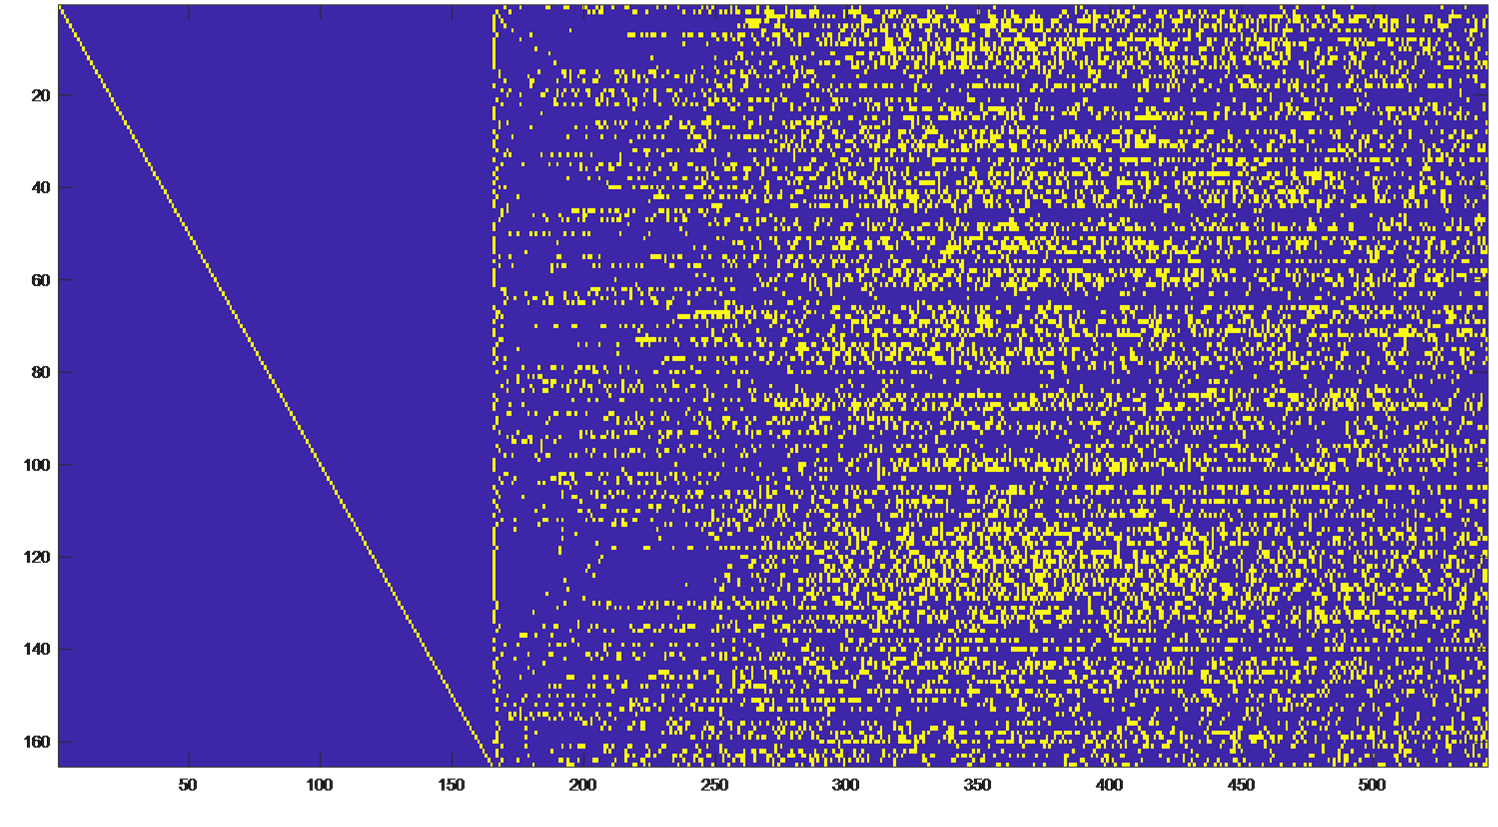
\includegraphics[width=0.9\textwidth]{SectionLetsMath/prescriptive_fig/fig_columnsGeneration.png}
\captionsetup{type=figure}
\caption{Evolution of a column generation algorithm.}
\label{fig_columnsGeneration}
\end{figure}

\section{Discrete event simulation}
Discrete event simulation (DES) is a problem-oriented technique which virtualises an entire system (products, resources, material handling system) and simulates the effect of the production to measure the efficiency of the entire system and get an estimate of some parameters as queues and takt-time dynamically. A DES model, as well as its outcomes,  is hard to generalise to multiple scenarios.

\section{Multiple decisions or decision-makers}
All the methods presented in this chapter are linked to a single objective and a single decision-maker. They can be easily generalised into multiple decision-making techniques using, for example, multi-objective optimisation. Nevertheless, when the information on the decision or the decision itself is distributed among different actors, there are different techniques (as game theory agent-based theory) which results adequate for this type of problems. The following section will focus on the decision problem where the final decision is in charge of a single decision-maker. For this reason, we will not use these techniques.